\clearpage
\section{Osnovni pojmovi i sistemi u igrama}
\label{sec:Section_Name}

\subsection{Game Loop}
Klju\v{c}na ta\v{c}ka izvr\v{s}avanja igre jeste glavna petlja igre (eng. game loop).
Jednom kada je igra pokrenuta sve ono \v{s}to je vidljivo korisniku, grafika, 
zvuk, interakcija procesira se kroz glavnu petlju. U tom jednom prolazu petlje koji
nazivamo \emph{tick} ili \emph{frame} de\v{s}ava se iscrtavanje grafike, reagovanje na 
korisni\v{c}ki unos (unos sa tastature ili putem mi\v{s}a ili nekih drugih perifernih ure\dj aja) 
te reakcija sveta na zadate promene... odnosno, ovde se de\v{s}ava sve, zato je glavna 
petlja srce same igre. Modernije arhitekture dozvoljavaju odre\dj eni stepen paralelizacije
nekih procesa, pa bi na primer iscrtavanje grafike moglo da se izdvoji u paralelan proces i sli\v{c}no.

\subsubsection{FPS}
FPS skra\'ceno od \emph{frames per second} je osnovna mera performansi igre. Ova mera kazuje nam
koliko je puta po sekundi mogu\'ce izvr\v{s}iti glavnu petlju. Ve\'ci broj je i bolji, pa tako igra
koja se izvr\v{s}ava na manje od 30 frejmova po sekundi nije prijatna za igranje
i doga\dj a se takozvano \emph{seckanje}, odnosno objekti se ne pomeraju glatko kako bi trebalo
ve\'c iscepkano \v{s}to naru\v{s}ava celokupan do\v{z}ivljaj igranja. Nizak FPS mo\v{z}e
da bude rezultat lo\v{s}e napisanog koda ili prosto zastarelog hardvera. Moderne igre se trude da 
se odr\v{z}e na 60 FPS.

\subsubsection{Update}
Update je funkcija koja se poziva upravo iz glavne petlje igre. To je funkcija koja je mo\v{z}e biti
definsana u MonoBehavior klasi. Update funkcija se poziva nad svakim objektom tipa MonoBehavior (ukoliko
je defini\v{s}e) ta\v{c}no jednom svakog frejma \cite{unitydocs}. Sva promenljiva pona\v{s}anja objekta
mogu se definisati ovde.

\subsubsection{FixedUpdate}
Sli\v{c}no funkciji Update, i ova funkcija se poziva periodi\v{c}no ali ne svakog frejma, ve\'c 
na fiksno vreme svake 0.02 sekunde \cite{unitydocs}. Prema uputstvima iz dokumentaicje,
u ovoj funkciji se mora raditi sve \v{s}to ima veze sa bilo kakvim izra\v{c}unavanjem fizike. U igri
se oslanjamo na Unity-jev sistem za fiziku za kretanje, pa \'cemo se dalje u tekstu detaljnije
baviti time.

\subsubsection{Vremena, klasa Time}
Jedna od bitnijih stavki u igrama jeste vreme. Merimo dve vrste vremena, koja o\v{c}itavamo iz klase \emph{Time}.

\emph{Time.time} je vreme koje je proteklo od pokretanja igre i ono je korisno
obi\v{c}no kada \v{z}elimo da ograni\v{c}imo izvr\v{s}avanje nekog dela koda vremenski.
Na primer, ne \v{z}elimo da neprijatelji prebrzo ispaljuju metke na igra\v{c}a, te mo\v{z}emo meriti
vreme proteklo od prethodnog pucanja i proveriti da li je to vreme ve\'ce od neke konstante
koja nam predstavlja minimalan vremenski interval izme\dj u dva pucnja.

\emph{Time.deltaTime} ~\ref{fig:deltatime} je vreme za koje se izvr\v{s}io prethodni frejm. Ovo je jako bitna stavka,
i potrebno nam je kada imamo bilo kakvu promenu stanja u igri koja je vidljiva (na primer, kretanje). 

\begin{center}
    \begin{figure}
        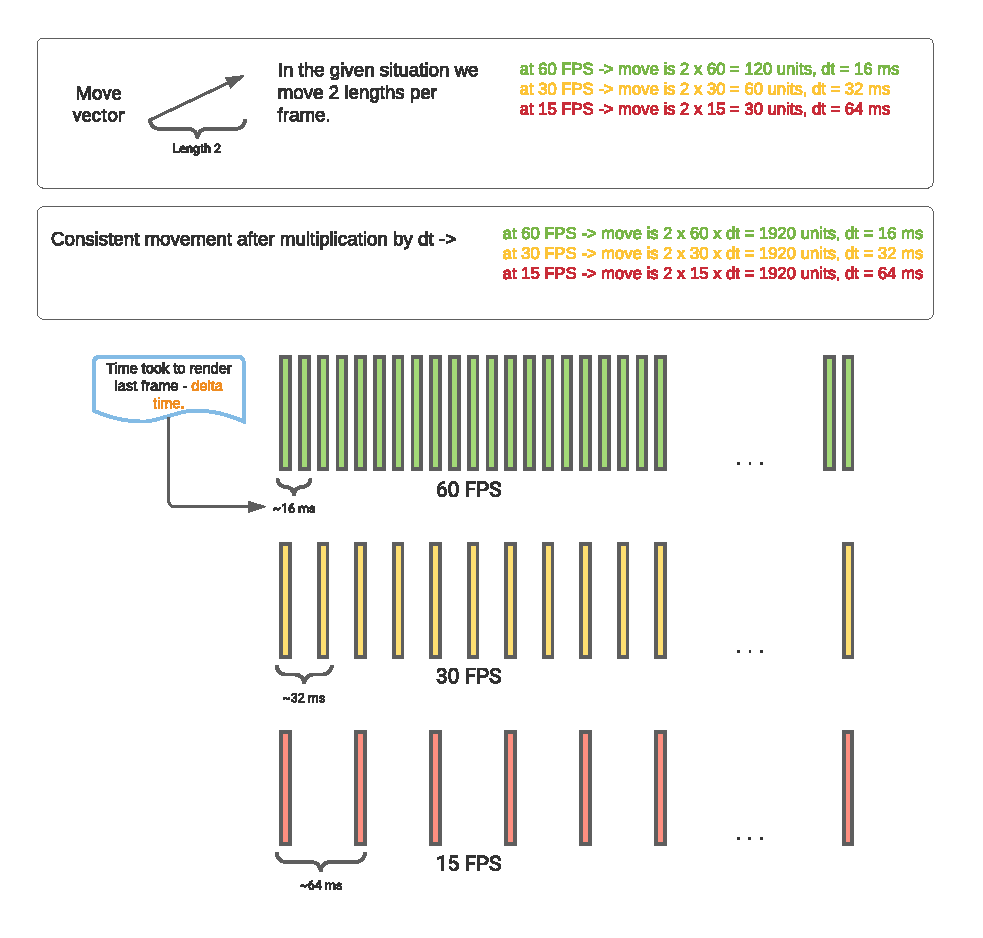
\includegraphics[width=1\textwidth]{Figures/DeltaTime.pdf}
        \caption{DeltaTime obja\v{s}njenje}
        \label{fig:deltatime}
    \end{figure}
\end{center}

\subsection{Obrasci (eng. design patterns)}
\subsubsection{"Singleton" obrazac}
\subsubsection{"Command" obrazac}
